\documentclass[12pt,conference,onecolumn]{IEEEtran}
\usepackage{diagbox}
\usepackage{graphicx}
\usepackage{amsmath}
\usepackage{amsfonts}
\usepackage{algpseudocode}
\usepackage{algorithm}
\usepackage{subfigure}
\usepackage{tikz}
% \usepackage[linesnumbered,ruled,vlined]{algorithm2e}
\usepackage{epsfig}
% \usepackage{pst-grad} % For gradients
% \usepackage{pst-plot} % For axes
\usepackage{cite}
\usetikzlibrary{shapes}
\usetikzlibrary{arrows,automata}
\usetikzlibrary{positioning}
\usetikzlibrary{patterns}
\usetikzlibrary{backgrounds}
\newtheorem{theorem}{Theorem}
\newtheorem{proposition}{Proposition}
\newtheorem{definition}{Definition}
\newtheorem{lemma}{Lemma}
\newtheorem{corollary}{Corollary}
\newtheorem{example}{Example}

%\renewcommand{\baselinestretch}{1}

\renewcommand{\ae}[1]{{\color{red}{#1}}}
\newcommand{\my}[1]{{\color{blue}{#1}}}
\newcommand{\old}[1]{{\color{green}{#1}}}
\begin{document}  
\title{Schedulability Analysis for Dual Priority Scheduling}  
\maketitle  


According to Baruah (2003, Dynamic- and Static-priority Scheduling of Recurring Real-time Tasks, Theorem~3), $\tau_i$ is schedulable on a single processor using static priority if and only if for each absolute deadline of a job  $d_{i,k}$ where $k\in N$, there exists an interval $d_{i,k-1}\leq t'\leq d_{i,k}$ for which the following condition holds:
\begin{equation}
dbf(\tau_i,t)+\sum_{\tau_j\in\{hp_i\}}rbf_i(\tau_j,t')\leq t	
\end{equation} 

Here the demand bound function captures the maximum execution demand of $\tau_i$ for a time interval length $t$ if it is to meet all deadlines.
\begin{equation}
dbf(\tau_i,t)=\left(\lfloor \frac{t-D_i}{T_i}\rfloor+1\right)\times C_i
\end{equation} 


On the other hand, the request bound function  $rbf_i(\tau_j,t')$ denotes the maximum amount of time for which $\tau_j$ could \textbf{deny the processor} to lower priority task $\tau_i$ over some interval length of $t'$. \\\\



\section{Dual Priority}

Given a task system $\tau=\{\tau_1,\tau_2,\ldots, \tau_n\}$, we first make the following \textbf{assumptions}:
\begin{enumerate}
	\item Each task  $\tau_i$ has a original priority $n+i$ and a promotion priority $i$.
	\item Each task has a fixed promotion point $p_i$. The concerned job $J_{i,k}$ has its promotion point $P_i=r_{i,k}+p_i$.
\end{enumerate}

\textbf{Difference:} Compared with static priority scheduling, each task has two tasks, and hence $\tau_{i+|a|}$ can also interfere task $\tau_i$.  However it is hard to exactly quantify the interference from other tasks unless \ae{we assume all previous jobs with deadline before  $t=d_{i,k}$ are meet to bound the maximum interference.}

% \textbf{Problem:} we need assume  $\tau_{i+|a|}$ meets deadline when analyze $\tau_i$
% % \section{}
% \section{Request bound function $rbf_i(\tau_j,t')$ when $j\leq i$}



% \begin{enumerate}
	% \item \textbf{Case 1: $t'\leq \lfloor t/T_j \rfloor T_j$ (e.g., $t_1'$)}. 
	% \item 	 \textbf{Case 2: $t'>\lfloor t/T_j \rfloor T_j$ (e.g., $t_2'$)}. 
	% \item \textbf{Case 1.1: Case 1 \& $P_j\leq P_i$}
	% \item \textbf{Case 1.2: Case 1 \& $P_j> P_i$}
	% \item \textbf{Case 2.1: Case 2 \& $P_i\leq t'\leq P_j$}
	% \item \textbf{Case 2.2: Case 2 \& $P_i\leq P_j\leq t'$}
	% \item \textbf{Case 2.3: Case 2 \& $P_i>P_j$}
% \end{enumerate}
\begin{figure}[h!]
 \centering
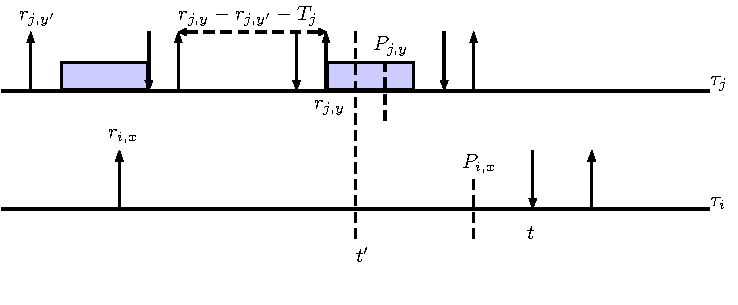
\includegraphics[scale=1]{Figure/C1}  
\caption{$ P_j\leq P_i$}
  \label{fig:p3}
\end{figure}
\begin{itemize}[\textbf{Property and Notations}]
	\item $n_j=\lfloor \frac{t'}{T_j}\rfloor$.
	\item $r_j=n_j\times T_j$
	\item   $P_j=n_j\times T_j+p_j$ denotes the promotion point of the last job we concern. For all other previous jobs we assume full interference.
	\item $P_i=t-(D_i-p_i)$ the last job's promotion point.
	\item $r_i=P_i-p_i$
	\item $[a]_0=\max(a,0)$
\end{itemize}


\subsection{$j\leq i$}
\textbf{Case 1 ( $P_j\leq P_i$):} 

The promotion point of $P_i$ is greater than $P_j$, and hence $\tau_i$ always has lower priority than $\tau_i$. Thus

	\begin{equation}
		rbf_i(\tau_j,t')=\lfloor \frac{t'}{T_j} \rfloor C_j +\min(C_j,t'-r_j)
	\end{equation}




\textbf{Case 2 ( $P_j> P_i$):} $\tau_i$ will not be interference by $\tau_j$ during $[P_i,P_j]$:
\begin{figure}[h!]
 \centering
\includegraphics[scale=1]{Figure/C2}  
\caption{$P_j> P_i$}
  \label{fig:p3}
\end{figure}
	\begin{equation}
		rbf_i(\tau_j,t')=\lfloor \frac{t'}{T_j} \rfloor C_j +\min\left(C_j,t'-r_j-\left(\min\{t',P_j\}-\max\{r_j,P_i\}\right)\right)
	\end{equation}


% \textbf{Summary} ($t'\leq \lfloor t/T_j \rfloor T_j)$:
% 	 	\begin{equation}
% 		rbf_i(\tau_j,t')=\lfloor \frac{t'}{T_j} \rfloor C_j +\min\left(C_j,t'-\lfloor \frac{t'}{T_j} \rfloor T_j-\left\{P_j-P_i\right\}_0\right)
% 	\end{equation}


% \subsection{B}

% \textbf{Case 3.1: ($t'>\lfloor t/T_j \rfloor   T_j\wedge t'\leq P_i\leq P_j$)}  $\tau_j$ has higher priority than $\tau_i$ during $\left [ \left\lfloor  t'/T_j \right\rfloor T_j, t'\right ]$

% \begin{equation}
% 		rbf_i(\tau_j,t')=\lfloor \frac{t'}{T_j} \rfloor C_j +\min(C_j,t'-\lfloor \frac{t'}{T_j} \rfloor T_j)
% 	\end{equation}

% \textbf{Case 3.2: ($t'>\lfloor t/T_j \rfloor T_j\wedge P_i\leq t'\leq P_j$)}  $\tau_j$ has higher priority than $\tau_i$ during $\left [ \left\lfloor  t'/T_j \right\rfloor T_j, P_i\right ]$
% 	\begin{figure}[h!]
%  \centering
% \includegraphics[scale=1]{Figure/21}  
% \caption{$t'>\lfloor t/T_j \rfloor T_j\wedge P_i\leq t'\leq P_j$}
%   \label{fig:p3}
% \end{figure}

% 	\begin{equation}
% 		rbf_i(\tau_j,t')=\lfloor \frac{t'}{T_j} \rfloor C_j +\min(C_j,\max(0,P_i-\lfloor \frac{t'}{T_j} \rfloor T_j))
% 	\end{equation}


% \textbf{Case 3.3: ($t'>\lfloor t/T_j \rfloor T_j\wedge P_i\leq P_j\leq t'$)}   $\tau_j$ has higher priority than $\tau_i$ during $\left [ \left\lfloor  t'/T_j \right\rfloor T_j, P_i\right ]$ and $[P_j,t']$
% 	\begin{figure}[h!]
%  \centering
% \includegraphics[scale=1]{Figure/22}  
% \caption{$t'>\lfloor t/T_j \rfloor T_j\wedge P_i\leq P_j\leq t'$}
%   \label{fig:p3}
% \end{figure}
% 	\begin{equation}
% 		rbf_i(\tau_j,t')=\lfloor \frac{t'}{T_j} \rfloor C_j +\min(C_j,\max(0,P_i-\lfloor \frac{t'}{T_j} \rfloor T_j)+t'-P_j)
% 	\end{equation}

% \textbf{Summary of Case 3} ($t'> \lfloor t/T_j \rfloor T_j\wedge P_i\leq P_j)$:
% 	 	\begin{equation}
% 			rbf_i(\tau_j,t')=\lfloor \frac{t'}{T_j} \rfloor C_j +\min(C_j,\{\min(P_i,t')-\lfloor \frac{t'}{T_j} \rfloor T_j\}_0+\{t'-P_j\}_0)
% 	\end{equation}

% \textbf{Case 4:  ($t'>\lfloor t/T_j \rfloor T_j\wedge P_i> P_j$)}   The promotion point of $P_i$ does not work at all. Thus
% 		\begin{figure}[h!]
%  \centering
% \includegraphics[scale=1]{Figure/23}  
% \caption{$t'>\lfloor t/T_j \rfloor T_j\wedge P_i> P_j$}
%   \label{fig:p3}
% \end{figure}
% 	\begin{equation}
% 		rbf_i(\tau_j,t')=\lfloor \frac{t'}{T_j} \rfloor C_j +\min(C_j,t'-\lfloor \frac{t'}{T_j} \rfloor T_j)
% 	\end{equation}





\section{Request bound function $rbf_i(\tau_j,t')$ when $j> i$}
 

% We define the following cases.
% \begin{enumerate}
% 	\item \textbf{Case 3: $P_i\leq P_k$)}. 
% 	\item \textbf{Case 4: $P_k\leq t'\leq P_i$)}. 
% 	\item \textbf{Case 5: $P_k\leq P_i\leq t'$}. 
% \end{enumerate}
% \textbf{Case 1 ($t'\geq \lfloor \frac{t'}{T_k} \rfloor T_k+D_k\wedge P_i\leq P_k$)}: $\tau_k$ will not interference $P_i$ at all. 
\textbf{Case 1 ($P_i\leq P_j$)}: $\tau_k$ will not interference $P_i$ at all. 

% However we should assume all deadlines before $t'$ is meet. whether we should assume it is meet.
	\begin{figure}[h!]
 \centering
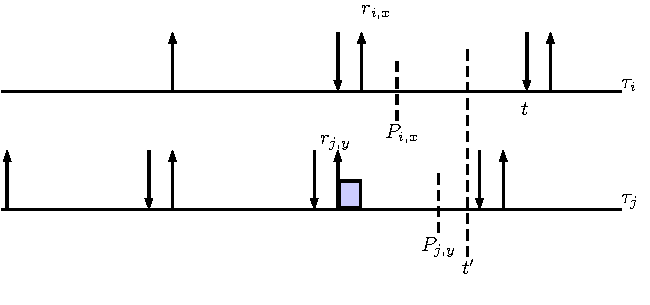
\includegraphics[scale=1]{Figure/C3}  
\caption{$P_i\leq P_j$}
  \label{fig:p3}
\end{figure}
		\begin{equation}
		rbf_i(\tau_j,t')=(\lfloor \frac{t'}{T_j} \rfloor)\times C_j
	\end{equation}



% \textbf{Case 2 ($t'<\lfloor \frac{t'}{T_k} \rfloor T_k+D_k\wedge P_i\leq P_k$)}: $\tau_k$'s last job can not interference $\tau_i$.


%  % interference during $\lfloor t'/T_k\rfloor T_k$ to $\lfloor t/T_i\rfloor T_i$

% 	\begin{figure}[h!]
%  \centering
% \includegraphics[scale=1]{Figure/32}  
% \caption{$t'<\lfloor \frac{t'}{T_k} \rfloor T_k+D_k\wedge P_i\leq P_k$}
%   \label{fig:p3}
% \end{figure}
	% 	\begin{equation}
	% 	rbf_i(\tau_k,t')=(\lfloor \frac{t'}{T_k} \rfloor) C_k+   \min\left(C_k, \max\left(0,\lfloor t/T_i\rfloor T_i-\lfloor t'/T_k\rfloor T_k\right)\right)
	% \end{equation}

	% \begin{equation}
	% 	rbf_i(\tau_k,t')=(\lfloor \frac{t'}{T_k} \rfloor)\times  C_k
	% \end{equation}


% $t'<\lfloor \frac{t'}{T_k} \rfloor T_k+D_k\wedge
\begin{enumerate}
	\item Distance between $P_i$ to $P_j$ is $P_i-P_j$. 
	\item Distance between $r_i$ to $P_j$ is $P_i-p_i-P_j$.
\end{enumerate}



{
\textbf{Case 2.1 ($P_i-P_j\leq p_i$)}: $\tau_j$ will  interference  $\tau_i$ during $[P_j,\min(t', P_i)]$.
	\begin{equation}
		rbf_i(\tau_j,t')=(\lfloor \frac{t'}{T_j} \rfloor) C_j+\min\left(C_j,\min(t', P_i)-P_j\right)
	\end{equation}


\textbf{Case 2.2 ($P_i- P_j>p_i $)}: Then during $P_j$ to $r_i$ there are $FI=[\lfloor \frac{P_i-p_i-P_j}{T_i}\rfloor \times (p_i)]_0$ full interference slack.

Then $P_{i,k-n}$ is $P_i-\lfloor \frac{P_i- p_i-P_j}{T_i} \rfloor \times T_i-T_i$, and the left carry-in interference slack is $CI=[P_{i,k-n}-P_j]_0$
} 

	\begin{figure}[h!]
 \centering
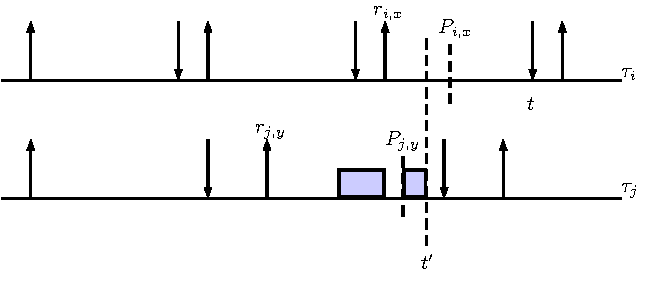
\includegraphics[scale=1]{Figure/C4}  
\caption{$ P_i>P_i$}
  \label{fig:p3}
\end{figure}
% 		\begin{equation}
% 		rbf_i(\tau_k,t')=(\lfloor \frac{t'}{T_k} \rfloor) C_k+\min\left(C_k,\max\left(0,\lfloor t/T_i\rfloor T_i-\lfloor t'/T_k\rfloor T_k\right)+\min(t',P_i)-\max(\lfloor t'/T_k\rfloor T_k,P_k)\right)
% 	\end{equation}


\begin{equation}
		rbf_i(\tau_k,t')=(\lfloor \frac{t'}{T_j} \rfloor) C_j+\min(C_j, \min(t', P_i)-r_{i}+FI+CI)
\end{equation}


% \textbf{Case 5:} interference happens during $[P_K,P_i]$, 
% 		\begin{equation}
% 		rbf_i(\tau_k,t')=\lfloor \frac{t'}{T_k} \rfloor C_k+\min(C_k,P_i-P_k)
% 	\end{equation}
\section{Summary of Equations}

% The rbf for $\tau_j$ with $T_j\leq T_i$:
% \begin{enumerate}
% \item ($t'\leq \lfloor t/T_j \rfloor T_j\wedge P_j\leq P_i)$
% \item ($t'\leq \lfloor t/T_j \rfloor T_j\wedge P_j> P_i)$
% \item ($t'> \lfloor t/T_j \rfloor T_j\wedge P_i\leq P_j)$)
% \item ($t'>\lfloor t/T_j \rfloor T_j\wedge P_i> P_j$)
% \end{enumerate}


Equation when $j<i$
\begin{equation}
\label{eqn:unnecessary}
\begin{split}
rbf_i(\tau_j,t')=
\begin{cases}
\lfloor \frac{t'}{T_j} \rfloor C_j +\min(C_j,t'-r_j)&\mbox{if}~ P_j\leq P_i\\
\lfloor \frac{t'}{T_j} \rfloor C_j +\min\left(C_j,t'-r_j-\left(\min\{t',P_j\}-\max\{r_j,P_i\}\right)\right)&\mbox{if}~ P_j>P_i
\end{cases}
\end{split}
\end{equation}


Equation when $j>i$
\begin{equation} 
\label{eqn:unnecessary}
\begin{split}
rbf_i(\tau_j,t')=
\begin{cases}
(\lfloor \frac{t'}{T_j} \rfloor)\times C_j&\mbox{if~} P_i\leq P_j\\
(\lfloor \frac{t'}{T_j} \rfloor) C_j+\min\left(C_j,\min(t', P_i)-P_j\right)&\mbox{if~}P_i-P_j\leq p_i\\
(\lfloor \frac{t'}{T_j} \rfloor) C_j+\min(C_j, \min(t', P_i)-r_{i}+FI+CI)&\mbox{if~}P_i- P_j>p_i
\end{cases}
\end{split}
\end{equation}
\section{Upper bound of t}
\begin{align*}
f_i(t,t')&=dbf(\tau_i,t)+\sum_{\tau_j\in\{\tau-\tau_i\}}rbf_i(\tau_j,t')\\
		&\leq t\times u_i+(\lfloor \frac{t'}{T_j} \rfloor+1)C_j\leq U\times t+\sum_{\tau_j\in\{\tau-\tau_i\}}C_j\\
	&\mbox{Suppose there exists an t such that}~f_i(t_F,t')>t_F,~\mbox{it must be that}\\
	&U\times t_F+\sum_{\tau_j\in\{\tau-\tau_i\}}C_j>t_F\Rightarrow t_F\leq \frac{\sum_{\tau_j\in\{\tau-\tau_i\}}C_j}{1-U}
\end{align*}



\end{document}  